% Szglab4
% ===========================================================================
%
\chapter{Szkeleton tervezése}

\thispagestyle{fancy}

\section{A szkeleton modell valóságos use-case-ei}

\subsection{Use-case diagram}

\begin{figure}[h]
\begin{center}
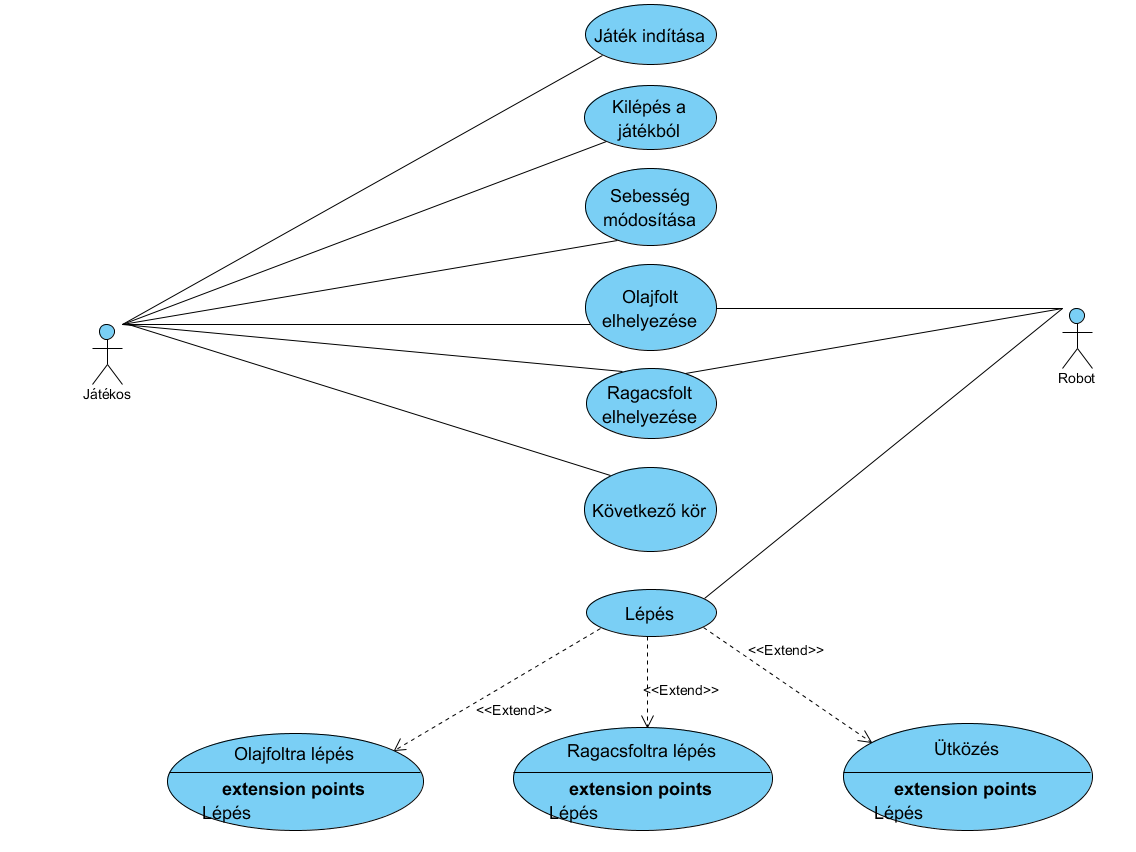
\includegraphics[width=17cm]{chapters/chapter05/use_case.png}
\caption{x}
\label{fig:SzkeletonUseCase}
\end{center}
\end{figure}

\subsection{Use-case leírások}



\usecase{Játék indítása}{Az egyik játékos elindítja a versenyt.}{Felhasználó}{A program menüjéből a felhasználó kiválasztja a Start game funkciót.}

\usecase{Kilépés a játékból}{A felhasználók ki tudnak lépni a játékból.}{Felhasználó}{Ha a játék közben egy játékos úgy dönt, hogy ki szeretne lépni, akkor ezt tudja jelezni és megsemmisül a hozzá tartozó robot.}

\usecase{Sebesség módosítása}{A robot sebesség vektora módosul.}{Játékos, Robot}{Egy játékos megváltoztatja saját robotjának a sebességét, tetszőleges irányú egységvektorral.}

\usecase{Olajfolt elhelyezése}{A robot egy olajfoltot hagy maga után.}{Játékos, Robot}{A játékos utasítására a robot elhelyez egy olajfoltot azon a cellán, amelyiken épp áll.}

\usecase{Ragacsfolt elhelyezése}{A robot egy ragacsfoltot hagy maga után.}{Játékos, Robot}{A játékos utasítására a robot elhelyez egy ragacsfoltot azon a cellán, amelyiken épp áll.}

\usecase{Következő kör}{Léptetés egy körrel.}{Játékos}{Ha minden játékos kiadta a kívánt utasításokat a robotoknak, akkor a kör befejeződik, s egy új kezdődik.}

\usecase{Kiesés a játékból}{Egy robot megsemmisülése.}{Robot}{Ha két robot ütközik, s nincs megfelelő cella számukra, akkor a két robot meghal és kiesik a játékból. Ha egy robot leugrik a kijelölt pályáról, akkor az szintén kiesik a játékból.}

\usecase{Játék megnyerése}{Egy robot megnyeri a játékot.}{Robot}{Ha egy robot marad már csak a pályán, akkor az a robot nyer. Ha elfogy a körök száma, akkor a legnagyobb távolságot megtett, életben maradt robot nyer.}

\usecase{Lépés}{A robot megteszi a lépését.}{Robot}{A robot tovább halad a pályán a megadott sebességvektorral.}

\usecase{Olajfoltra lépés}{A robot rálép egy olajfoltra.}{Robot}{Egy robot egy olajfoltos cellára kénytelen lépni, ezáltal a következő körben a sebessége nem módosítható.}

\usecase{Ragacsfoltra lépés}{A robot rálép egy ragacsfoltra.}{Robot}{Egy robot egy ragacsfoltos cellára kénytelen lépni, ezáltal a sebessége megfeleződik.}

\usecase{Ütközés}{A robotok ütköznek.}{Robot}{Két robot azonos cellára lép, így összeütköznek. Ha a robot egy olyan cellára lép, amelyen már áll egy robot, akkor az ott álló robot továbblép egy véletlenszerűen meghatározott szomszédos cellára. Ha nincs ilyen üres cella, akkor mindkét robot megsemmisül.}


\section{A szkeleton kezelői felületének terve, dialógusok}
\comment{A szkeleton által elfogadott bemenetek , valamint a szöveges konzolon megjelenő kimenetek. A kiemenet formátuma olyan kell legyen, ami alapján a működés összevethető a korábbi szekvencia-diagramokkal.}

\section{Szekvencia diagramok a belső működésre}
\comment{A szkeletonban implementált szekvenciadiagramok. Tipikusan egy use-case egy diagram. Ezek megegyezhetnek a korábban specifikált diagramokkal, de az egyes életvonalakat (lifeline) egyértelműen a szkeletonban példányosított objektumokhoz kell tudni kötni. Azt kell megjeleníteni, hogy a szkeletonban létrehozott objektumok egymással hogyan fognak kommunikálni.}

\section{Kommunikációs diagramok}
\comment{A szkeletonban, az egyes szkeleton-use-case-ek futása során létrehozott objektumok és kapcsolataik bemutatására szolgáló diagramok. Ezek alapján valósítják meg a szkeleton fejlesztői az inicializáló kódrészleteket.}
